
\chapter*{Doppler-freie Spektroskopie von \ch{Rb}}
	
\section{Motivation und Ziele}

\begin{itemize}
	\item Dieses Experiment zeigt, wie die Energie der Zustände in Atomen und die Übergänge zwischen ihnen mit Hilfe der Quantenmechanik korrekt beschrieben werden können. Es ist ein Beispiel für quantenmechanische Drehimpulsaddition in Aktion.
	
	\item Im Experiment werden Energieabstände zwischen Übergängen in Rubidiumatomen gemessen, die viel kleiner sind als die Energie des Übergangs selbst. Dabei macht man sich den Umstand zunutze, dass man nur relative, nicht aber absolute Energien genau messen muss.
	
	\item Die zu messenden Energieabstände sind so klein, dass die thermische Bewegung der Atome zu einer Doppler-Verschiebung führt, die alles überdecken würde. Im Experiment verwenden wir eine nichtlineare optische Methode, um nur Atome zu beobachten, die sich  relativ zum Laserstrahl nicht bewegen.
\end{itemize}


\newcommand{\auftraege}{%
\section{Arbeitsaufträge}

\begin{itemize}
	\item Messen Sie ein Doppler-freies Spektrum der D2-Linien von Rubidium und geben Sie die zugehörigen Übergänge an.
	\item Bestimmen Sie den Dipol- und den Quadrupol-Term der Hyperfeinstrukturkonstanten (inkl. Messunsicherheit).
	\item Messen Sie das Doppler-verbreiterte Absorptionsspektrum bei verschiedenen Temperaturen und modellieren Sie die Linienform.
	\item Bonus: Untersuchen Sie den Einfluss der Leistung von Abfrage- und Sättigungsstrahl.
	\item Bonus: Versuchen Sie, möglichste schmale Linien zu erreichen. 
	\item Bonus: Vergleichen Sie die Amplituden der Linien mit einem passenden Modell.
\end{itemize}
}

 \auftraege

\nocite{Hertel2015,Meschede,DemtL1,DemtL2,Gert,Dem3,Dem4}

\section{Rubidium}
	

Rubidium (\ch{Rb}) ist ein Alkalimetall und steht im Periodensystem in der ersten Hauptgruppe. Die Elektronenkonfiguration ist [\ch{Kr}]5s$^1$. Rubidium hat also ein 'Leuchtelektron' und ist damit sehr ähnlich zu  Wasserstoff. 

%\paragraph{Zur Vorbereitung} schauen Sie bitte in Ihre Notizen zur Quantenmechanik und Atomphysik zu den Stichworten Drehimpuls-Addition, Spin-Bahn-Kopplung, Feinstruktur-Aufspaltung, Hyperfeinstruktur-Aufspaltung

In diesem Experiment untersuchen Sie die Anregung dieses 5s-Elektrons in die p-Schale. Dabei ändert sich die Drehimpulsquantenzahl des Elektrons von $l=0$ nach $l=1$. Aufgrund der Spin-Bahn-Kopplung spaltet sich der Zustand $l=1$ in zwei Zustände auf, die sich in der relativen Orientierung von Elektronenspin und Bahndrehimpuls unterscheiden, was zu einem unterschiedlichen Gesamtdrehimpuls $j$ führt.

Die meisten Atome haben mehr als ein Elektron in der äußeren Schale, so dass man Spin, Bahn- und Gesamtdrehimpuls aller Elektronen addiert und mit den großen Symbolen bezeichnet. Ich benutze $S$, $L$ und $J$ als Bezeichnung der Quantenzahl und 
$\mathbf{S}$, $\mathbf{L}$ und $\mathbf{J} = \mathbf{L} + \mathbf{S}$ als Operator. Diese drei Quantenzahlen und die Hauptquantenzahl $n=5$ werden im spektroskopischen Symbol der Form $n^{2S+1}L_J$ kodiert. Der Grundzustand ist $5^2S_{1/2}$. Die zwei angeregten Zustände sind $5^2P_{1/2}$ und $5^2P_{3/2}$. Die Übergänge werden als D1- bzw. D2-Linien bei den Wellenlängen 794,98 nm (D1) und 780,24 nm (D2) bezeichnet.

\begin{marginfigure}
	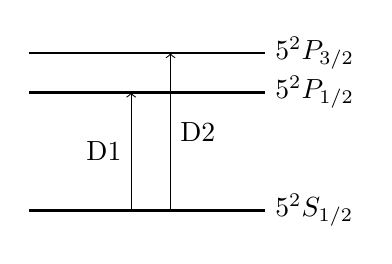
\begin{tikzpicture}
		\draw[thick] (0, -2) -- (3, -2) node[right] { $5^2P_{3 / 2}$ };
		\draw[thick] (0, -2.5) -- (3, -2.5) node[right] { $5^2P_{1 / 2}$ };
		\draw[thick] (0, -4) -- (3, -4) node[right] {$5^2S_{1 / 2}$};

		\draw[->] (1.3,-4) to node[left] {D1} (1.3, -2.5); 
		\draw[->] (1.8,-4) to node[right]{D2} (1.8, -2);
	\end{tikzpicture}
	\caption{D1- und D2-Linie von Rubidium.}	
	\label{D-Linie}
\end{marginfigure}

Der Energieunterschied zwischen $5^2P_{1/2}$ und $5^2P_{3/2}$ ist jedoch für den Versuchsaufbau viel zu groß. Wir betrachten nur einen dieser beiden Übergänge, aus technischen Gründen\sidenote{siehe CD Player} den höherenergetischen nach $5^2P_{3/2}$, also die D2-Linie. Nun kommt aber der Kernspin $\mathbf{I}$ ins Spiel. Auch der Kernspin ist ein magnetisches Moment, und die Orientierung des Kernspins relativ zu den anderen magnetischen Momenten liefert einen Energiebeitrag, die Hyperfeinstruktur, ganz analog zur oben besprochenen Feinstruktur. Aus der Kopplung mit dem elektronischen Gesamtdrehimpuls $\mathbf{J}$ ergibt sich somit ein Gesamtdrehimpuls $\mathbf{F} = \mathbf{J} + \mathbf{I}$.

Der Kernspin von Rubidium beträgt je nach Isotop $I = 5/2$ (\ch{^{85}Rb}) oder $I = 3/2$ (\ch{^{857}Rb}). Somit kann $F$ je nach elektronischem Zustand und Isotop verschiedene Werte annehmen. Für den Grundzustand \ch{^{85}Rb} gilt $J = 1/2$ und $I = 5/2$, also $F = 2$ oder $F = 3$ (\ch{^{87}Rb}: $F = 1$ oder 2). Für den angeregten Zustand der D2-Linie ($5^2P_{3/2}$ ) kann $F$ jeden der Werte $1$, $2$, $3$ oder $4$ annehmen (\ch{^{87}Rb}: $F = 0$ bis $3$). Die Auswahlregeln sind analog zu denen des Gesamtdrehimpulses $\mathbf{J}$, d.h. $\Delta F=0,\pm 1$.

Die Wechselwirkung des Kernspins mit dem Elektron kann man analog der Spin-Bahn-Kopplung berechnen. Die Dipol-Wechselwirkung liefert
\begin{equation}
	\Delta E_{dipol} = A_{HFS} \, \mathbf{I} \cdot \mathbf{J} =	\frac{h \, A_{HFS}}{2} \, K
\end{equation}
mit $A_{HFS}$ der  magnetische Dipol-Konstante der Hyperfeinstruktur und  
\begin{equation}
K =  F( F+1) - I (I+1) - J(J+1) \quad .
\end{equation}
Falls der Kernspin $I > 1/2$ ist, und gleichzeitig die Ladungsverteilung der Elektronen einen Gradienten am Ort des Kerns liefert, was bei  $J > 1/2$ der Fall ist, dann kommt noch eine Quadrupol-Wechselwirkung hinzu:
\begin{equation}
	\Delta E_{quadrupol} = \hbar \,  B_{HFS}  \frac{\frac{3}{2} K (K+1)- 2 I (I+1) J (J+1)}%
	{ 4 I (2I -1)J(2J-1)} \quad .
\end{equation}
Dieser Term ist in der Amplitude kleiner, kann aber im Experiment nicht vernachlässigt werden.


\begin{table}
\begin{tabular}{rrr}
	 						&  \ch{^{85}Rb} 		& \ch{^{87}Rb} \\
$\nu_{D2}$  				& 384 230 406.4 MHz    &  384 230 484.5  MHz \\

$A_{HFS}$ für $5^2S_{1/2}$ & 1 011.9 MHz & 3 417.3  MHz \\
$A_{HFS}$ für $5^2P_{3/2}$ & 25.0 MHz     & 84.7 MHz \\
$B_{HFS}$ für $5^2P_{3/2}$ & 25.8 MHz     & 12.5 MHz \\
\end{tabular}
\caption{Relevante Konstanten zur Berechnung der Übergangsenergien, aus \cite{Data85,Data87}}
\label{tab:konstanten}
\end{table}

Damit haben wir alles, um das quantenmechanisch vorhergesagte Hyperfeinstruktur-Spektrum der D2-Linie von Rubidium zu berechnen. Abbildung \ref{sim_spectra} zeigt das Ergebnis auf einer absoluten Frequenz- bzw. Wellenlängenachse. Das Verhältnis des kleinsten Frequenzabstandes zur absoluten Frequenz beträgt etwa $10^{-7}$. Dies ist die erforderliche Auflösung eines Spektrometers, mit dem sowohl die absoluten Frequenzen / Wellenlängen als auch die Abstände der Übergänge bestimmt werden können. Gute Gitterspektrometer erreichen etwa $10^{-5}$ oder 0.02~nm. Daher gehen wir in diesem Experiment davon aus, dass die Wellenlänge des Übergangs grob bekannt ist (also ca. 780~nm) und messen nur die Abstände zwischen den Übergängen bzw. ein Spektrum mit einer willkürlichen Lage des Frequenznullpunkts.


\begin{figure}
	\inputtikz{\currfiledir sim_frequenz}

 \vspace*{5mm}

	\inputtikz{\currfiledir sim_wavelength}
	\caption{Lage der Übergänge auf einer absoluten Frequenz- bzw. Wellenlängenachse.}
	\label{sim_spectra}
\end{figure}




\begin{figure}
	\inputtikz{\currfiledir sim_frequenz_null}

	\caption{Lage der Übergänge auf einer relativen Frequenzachse mit willkürlichem Nullpunkt.}
	\label{sim_spectra_null}
\end{figure}


\paragraph*{Zur Vorbereitung}  Nur sehr selten ist die erste Messung erfolgreich. Sie werden verschiedene Parameter optimieren müssen. Daher ist es notwendig, die Messung sofort soweit auszuwerten, dass der Optimierungsbedarf erkannt werden kann.  In den 'Fragen zur Vorbereitung' werden Sie daher schrittweise eine Testmessung auswerten.

\begin{questions}
	\item Zeichnen Sie ein Diagramm, das die energetische Lage der relevanten Zustände und die erlaubten Übergänge skizziert. Geben Sie dabei sowohl die spektroskopische Bezeichnung als auch die Quantenzahlen an.
	\item Berechnen Sie im Experiment erwarteten Linien-Positionen und Linien-Abstände. Zur Kontrolle: der kleinste Abstand sollte 29.4~MHz betragen (ohne die unten eingeführten cross-over-peaks). \label{frage:peaks}
\end{questions}
	

\section{Laserspektroskopie}

Die Kernidee der Laserspektroskopie besteht darin, das Spektrum des Lichts nicht erst nach der Probe in einem Spektrometer möglichst genau zu bestimmen, sondern bereits die Probe mit einem Laser als Lichtquelle mit nur einer einzigen spektral schmalen Linie anzuregen. Die Frequenz dieser Laserlinien wird dann schrittweise verändert und jeweils die Transmission der Probe bestimmt, hier also die Transmission durch ein Rubidiumgas.

Im Experiment verwenden wir einen Halbleiterlaser, ähnlich dem in einem CD-Player. Der Strom fließt durch einen pn-Übergang, in dem Elektronen und Löcher rekombinieren und dabei Licht aussenden, ähnlich wie bei einer Leuchtdiode. Allerdings dient hier das Halbleitersubstrat als Laserresonator, in dem zum Beispiel die Endflächen verspiegelt sind. Bei unserem Laser handelt es sich um einen 'External Cavity Diode Laser' (ECDL). Hier ist eine der Endflächen entspiegelt und der benötigte Resonatorspiegel wird durch ein 'volume Bragg grating' gebildet\sidenote{nicht wie ein optisches Oberflächengitter, eher wie ein 3D-Kristall}, das bei 780,2~nm in einem etwa 0,2~nm breiten Spektralbereich besonders gut reflektiert.

In Lasern bilden sich Resonatormoden aus, wenn die Resonatorlänge genau ein ganzzahliges Vielfaches der halben Laserwellenlänge ist, d.h. es bilden sich Knoten auf den Spiegeln. Bei dem hier verwendeten Laser beträgt der Abstand dieser Moden im Frequenzraum etwa 7~GHz. Das spektrale Verstärkungsprofil des Lasers wird insbesondere durch die Reflektivität des Gitters so eingestellt, dass nur eine dieser Moden zu emittieren beginnt. Der Laser ist ein 'single mode' Laser.

Um die Frequenz des Lasers zu ändern, wird die Temperatur des Halbleiterkristalls verändert. Dadurch ändert sich sein Brechungsindex und damit die effektive Länge des Resonators, der Abstand zwischen den Moden wird geringfügig größer und die Lasermode schiebt sich durch das Verstärkungsprofil. Irgendwann erfährt die 7 GHz höhere oder tiefere Mode weniger Verluste. Der Laser springt auf diese Mode und ändert seine Frequenz schlagartig um den Modenabstand. Diese 'mode hops' begrenzen den Frequenzbereich, der einfach abgetastet werden kann.  Der Laser ist jedoch so gewählt, dass das Rubidium-Spektrum gerade noch hineinpasst.

\begin{marginfigure}
	%\includegraphics*[width=\textwidth]{bilder/sacher_tuning.png}
	\inputtikz{\currfiledir laser_wavelength}
	\caption{Exemplarischer Zusammenhang zwischen Laserwellenlänge und Laserstrom (aus dem Datenblatt des Herstellers).}
\end{marginfigure}

Die Temperatur des Halbleiterkristalls kann auf zwei Arten verändert werden: über den Strom, der durch den Kristall fließt, und über ein angebrachtes Peltier-Element. Die Steuerung über den Strom ist viel schneller und einfacher, ändert aber natürlich auch die Ausgangsleistung des Lasers und deckt nur einen relativ kleinen Spektralbereich ab. Das Peltier-Element ist langsamer, deckt aber einen größeren Bereich ab. Im Experiment muss also eine Kombination aus Peltier-Temperatur und Laserstrom gefunden werden, so dass die Laserfrequenz gerade die Peaks des Rubidium-Spektrums überdeckt. Erfahrungswerte können als Startwerte dienen, die konkreten Werte müssen jedoch täglich optimiert werden.


\section{Fabry-Pérot Interferometer}

Wir verstimmen die Frequenz des Lasers mit Hilfe des Stroms oder des Peltier-Elements und messen die Transmission durch das Rubidiumgas. Um daraus ein Spektrum zu erstellen, müssen wir zu jedem Zeitpunkt die Frequenz des Lasers kennen, die in der Nähe von $\nu_0 \approx 384 230$~GHz liegt. Ein 'Wave Meter' misst optische Frequenzen mit sehr hoher Genauigkeit, ist aber zu teuer und auch nicht notwendig. Relative Frequenzen sind für das Experiment ausreichend.

\begin{marginfigure}
	\inputtikz{\currfiledir Fabry_Perot}
	\caption{Transmission durch das Fabry-Perot-Interferometer. Bei etwa 109~mA und 115~mA sind Modensprünge zu erkennen. Der Abstand der Peaks entspricht dem FSR.}
\end{marginfigure}

Wir verwenden ein Fabry-Perot-Interferometer, um regelmäßige Marker auf der Frequenzachse zu erzeugen. Ein Fabry-Perot-Interferometer besteht aus zwei (teildurchlässigen) Spiegeln und entspricht damit einem Laserresonator. Es kommt zu konstruktiver Interferenz, wenn die Länge eines geschlossenen Stahlwegs im Resonators ein ganzzahliges Vielfaches der  Wellenlänge ist. Wird die Frequenz des Lasers variiert, kommt es periodisch zu konstruktiver und destruktiver Interferenz. Der spektrale Abstand wird hier freier Spektralbereich (engl. free spectral range, FSR) genannt und beträgt.
	\begin{equation}
	\Delta\nu_{FSR}=\frac{c_0}{L}  
	\end{equation}
mit der Lichtgeschwindigkeit $c_0$ und $L$ der Länge des Strahlwegs. Im Experiment verwenden wir einen konfokalen Resonator mit sphärischen Spiegel und gemeinsamen Brennpunkt. Dadurch ist die optische Weglänge im Resonator vier mal der Abstand der Spiegel,  so dass sich ein freier Spektralbereich von ca. 300 MHz ergibt. Im Experiment wird parallel zum Transmissionssignal durch das Rubidium-Gas die durch das Fabry-Perot-Interferometer transmittiert Leistung gemessen. Aus der periodischen Änderung dieser Leistung wird dann die relative Frequenzachse konstruiert.



% \begin{questions}
% 	\item Bestimmen Sie die Abstände der Linien im Beispiel-Datensatz (hier XXX). Um welche Übergänge handelt es sich?
% \end{questions}


\section{Doppler-Verbreiterung}

Im Prinzip hätten wir jetzt alles, was wir brauchen. Aber es gibt noch die Doppler-Verschiebung. Bewegt sich eine Atom mit der Geschwindigkeit  $v$ in Strahlrichtung, so ändert sich seine Absorptions-Frequenz aufgrund der Doppler-Verschiebung um $\Delta \nu$.
\begin{equation}
	\Delta \nu = \frac{v}{c_0} \, \nu_0
\end{equation}
mit der Ruhe-Frequenz $\nu_0$. Die Geschwindigkeit kommt  aus der  Maxwell-Boltzmann-Geschwindigkeitsverteilung $P(v)$
\begin{equation}
	P(v) = \sqrt{\frac{M}{2 \pi k_B T}} \, \exp \left (
	- \frac{M v^2}{2  k_B T}	
	\right) \quad .
\end{equation}
Insgesamt ergibt sich damit eine gaußförmige  Linie der Halbwertsbreite 
\begin{equation}
	 \Delta \nu_{doppler} = \nu_0 \, \sqrt{\frac{8 k_B T \ln 2} {M c^2}} \quad .
\end{equation}
Für Rubidium bei Raumtemperatur beträgt die Doppler-Verbreiterung etwa 500~MHz. Wenn wir einfach die Transmission des Laserstahls durch das Rubidiumgas bestimmen, werden wir nur vier Peaks von etwa 500~MHz Breite finden, aber die Details der Hyperfeinstruktur nicht auflösen können. Wir müssen also 'Doppler-frei' messen.


\begin{questions}
	\item Berechnen Sie das erwartete Doppler-verbreiterte Spektrum von Rubidium in der natürlichen Isotopenmischung.
	\label{FzV:doppler_theo}
\end{questions}


\section{Sättigung}

Bisher haben wir nur die Frequenz des D2-Übergangs in Rubidium betrachtet. Jetzt müssen wir auch die Übergangswahrscheinlichkeit diskutieren. Damit ein Rubidium-Atom ein Photon mit einer Wellenlänge von etwa 780~nm absorbieren kann, muss nicht nur die Wellenlänge genau passen, sondern das Atom muss sich auch im Grundzustand befinden. Dies ist zunächst bei allen Atomen der Fall. Unmittelbar nach der Absorption bleibt das Rubidium-Atom jedoch im angeregten Zustand und fällt nur mit der Rate 
\begin{equation}
	k_{decay} = \frac{1}{\tau} = \frac{1}{26.24~ns} = 38.1~MHz
\end{equation}
in den Grundzustand zurück. Die Anregungsrate $k_{ex}$ ist proportional zum Absorptionsquerschnitt $\sigma$ des Atoms bei dieser Wellenlänge und zur Laser-Intensität $I$
\begin{equation}
	k_{ex} = \sigma \frac{I}{h \nu} \quad .
\end{equation}
In die Ratengleichung für den Anteil $0 \le n \le 1$ aller Atome im Grundzustand geht die Anregungsrate $k_{ex}$ jedoch nur mit der Differenz $\Delta n = n - (1-n) = 2n -1$ der Besetzung im Grundzustand und im angeregten Zustand ein, da die stimulierte Emission der Absorption entgegenwirkt:
\begin{equation}
	\frac{d n}{dt} = - k_{ex} \, \Delta n + k_{decay} (1-n) = - k_{ex} \, \Delta n + k_{decay} \frac{1 - \Delta n}{2} \quad .
\end{equation}
 Im Gleichgewicht findet wir
\begin{equation}
	\Delta n = \frac{k_{decay}}{2 k_{ex}+ k_{decay}} = \frac{1}{1 + 2 k_{ex} \tau } = \frac{1}{1 + I / I_{sat}}
\end{equation}
mit der Sättigungsintensität $I_{sat}$
\begin{equation}
	I_{sat} = \frac{h \nu}{2 \sigma \tau } \quad .
\end{equation}
Für die D2-Linien von Rubidium beträgt $I_{sat} \approx 1 mW/cm^2$, wenn die Wellenlänge einem Übergang entspricht.
Wenn die Laserintensität $I$ klein ist, dann ist $\Delta n \approx 1 - I / I_{sat}$. Für $I = I_{sat}$ ist $\Delta n = 0.5$, d.h. ein Viertel aller Atome befindet sich im angeregten Zustand ($n=0.75$). Für sehr große Intensitäten geht $\Delta n$ gegen Null. Es befinden sich dann gleich viele Atome im Grundzustand wie im angeregten Zustand.

Die Absorption von Rubidiumgas kann durch das Lambert-Beer'sche Gesetz mit dem Absorptionskoeffizienten $\alpha$ beschrieben werden. Die transmittierte Leistung $P$ nimmt exponentiell mit der Länge $L$ der Probe ab:
\begin{equation}
	P = P_0  \, e^{- \alpha L} \quad . \label{eq:lambert_beer}
\end{equation}
Der Absorptionskoeffizienten $\alpha$ ist
\begin{equation}
	\alpha = \sigma  \, \rho  \, \Delta n
\end{equation}
mit der Teilchenzahldichte $\rho$ des Gases.


\begin{questions}
	\item Bei sehr niedriger Laserleistung werden im Peak 95\% des Lichts in der Gaszelle absorbiert. Berechnen Sie via Gl.~\ref{eq:lambert_beer} die Form des Doppler-verbreiterten Absorptionspektrums und vergleichen Sie mit Ihrem Ergebnis von Frage \ref{FzV:doppler_theo}.
\end{questions}


\section{Dampfdruckkurve und Teilchenzahldichte}

Rubidium ist ein Metall mit einem Schmelzpunkt von 39.30$^\circ$~C (312.45~K). In der Gaszelle befindet sich außer Rubidium kein anderes Gas. Die Rubidium-Konzentration im Gas wird durch den Dampfdruck bestimmt. Die Dampfdruckkurve hat die Form
\begin{equation}
    P = P_0 \, e^{- \frac{T_0}{T}}
\end{equation}
mit den Konstanten $P_0$ und $T_0$ aus nebenstehender Tabelle. 

\begin{margintable}
    \begin{tabular}{lll}
           & $P_0$ (GPa) & $T_0$ (K) \\
           fest  &  7.293   & 9705 \\
           flüssig  &  2.079  & 9302 \\
    \end{tabular}
	\caption{Parameter zur Dampfdruckkurve, aus \cite{Data85}.}
\end{margintable}



Die Teilchenzahldichte $\rho$ ergibt sich aus dem Dampfdruck über das ideale Gasgesetz. Die Teilchenzahldichte steigt also mit der Temperatur steil an.


\section{Sättigungsspektroskopie}

Die Sättigung eines atomaren Übergangs, d.h. die Verringerung des Absorptionskoeffizienten $\alpha$ durch die Verringerung der Besetzungsdifferenz $\Delta n$, steht im Mittelpunkt der Sättigungsspektroskopie.  Ein Pumpstrahl sättigt die mit ihm wechselwirkenden Atome. Durch den Dopplereffekt sind dies genau die Atome, die eine passende Frequenzverschiebung aufweisen. Sei $\omega_L$ die Laserfrequenz und $\omega_0$ die Frequenz des atomaren Übergangs (z.B. $\omega_0 > \omega_L$), dann sind dies genau die Atome mit der Geschwindigkeit $+v$ relativ zum Pumpstrahl, so dass
\begin{equation}
	\omega_0 = \omega_L \left( 1 - \frac{v}{c_0} \right)
\end{equation}
Für diese Atome mit der Geschwindigkeit $v$ ist nun der Absorptionskoeffizient $\alpha$ kleiner. Der entgegengesetzte, schwächere Abfragestrahl hat die gleiche Laserfrequenz. Wegen der entgegengesetzten Ausbreitungsrichtung passen hier aber nur die Doppler-verschobenen Atome mit der Geschwindigkeit $-v$ zur Laserfrequenz. Der Abfragestrahl erfährt daher zunächst keine Änderung des Absorptionskoeffizienten.

Liegt die Laserfrequenz jedoch innerhalb der natürlichen Linienbreite des Übergangs, d.h. $\omega_0 \approx \omega_L$, so wechselwirken beide Strahlen mit derselben Atompopulation, d.h. mit Atomen mit $v \approx 0$ (wobei $v$ die Geschwindigkeit entlang des Strahls ist. Senkrecht zum Strahl kann sie immer noch von Null verschieden sein). Variiert man die Frequenz der beiden Strahlen und zeichnet die Transmission des Abfragestrahls auf, so erhält man ein Doppler-verbreitertes Absorptionsprofil, solange die Laserfrequenz noch weit von der Frequenz des Übergangs entfernt ist. Am Übergang selbst entsteht ein \emph{Lamb-Dip} in der Absorption, d.h. eine stärkere Transmission, wenn beide Strahlen mit der gleichen Population wechselwirken. Die Breite des Lamb-Dip ist nur durch die natürliche Linienbreite begrenzt, nicht mehr durch die Doppler-Verbreiterung.

\begin{marginfigure}
	\inputtikz{\currfiledir Lamb_dip}
	\caption{oben: Ein Laser der Frequenz $\omega = \omega_0 (1 - v_0/c_0)$ brennt ein Loch in die ansonsten Maxwell-förmige Geschwindigkeitsverteilung der Atome im Grundzustand. unten: Dies führt zum Lamb-Dip im Absorptionsspektrum des gegenläufigen Abfrage-Strahls.}
\end{marginfigure}

Liegen mehrere atomare Übergänge innerhalb der Doppler-Verbreiterung, so erhält man für jeden Übergang Lamb-Dips in der Absorption. Zusätzlich findet man auch \emph{'cross over dips'} genau zwischen zwei atomaren Übergängen mit gemeinsamem Grundzustand. Bei dieser Laserfrequenz ist die Geschwindigkeit $+v$ geeignet, dass der Pumpstrahl einen der Übergänge antreibt und damit den Grundzustand entvölkert. Für den Abfragestrahl haben diese Atome die Geschwindigkeit $-v$, was in diesem Fall gerade dem anderen Übergang entspricht. Da dem Pump-Strahl zwei Übergänge zur Depopulation zur Verfügung stehen, erfährt der  Abfragestrahl  also auch hier eine reduzierte Absorption. Die cross-over peaks sind in erster Näherung doppelt so stark wie die direkten Übergänge.


\begin{questions}
	\item Ergänzen Sie Ihre vorhergesagten Peak-Positionen aus Frage \ref{frage:peaks} um die cross-over peaks.
\end{questions}
	

\section{Balanced Detector}

Ein störender Aspekt des Verstimmens der Laserfrequenz durch den Strom ist die sich ändernde Intensität. Diese kann durch 'balanced detection' eliminiert werden. Ein weiterer Laserstrahl durchläuft das Rubidiumgas parallel zum Abfragestrahl, aber ohne Überlappung mit dem Pumpstrahl. Dieser Referenzstrahl erfährt somit nur die übliche Doppler-Verbreiterung. Ein Detektor mit zwei Photodioden misst die Leistung in beiden Strahlen. Es wird jedoch nur die Differenz der Photoströme durch die beiden Dioden verstärkt. Eine synchrone Änderung oder Fluktuation der Leistung an beiden Dioden wird somit unterdrückt. Das Unterdrückungsverhältnis ('common mode rejection') beträgt etwa 30~dB, also einen Faktor 1000. Damit können kleine Unterschiede zwischen ansonsten sehr ähnlichen Signalen detektiert werden.

\begin{marginfigure}
	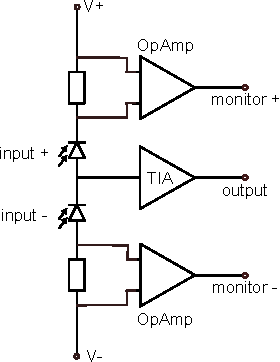
\includegraphics{bilder/balanced.pdf}
	\caption{Balanced detection. OpAmp: Operationsverstärker. TIA: Transimpedanzverstärker, also Strom-Spannungs-Wandler.}
\end{marginfigure}

Damit dies gut funktioniert, müssen die Leistungen im Abfrage- und Referenzstrahl möglichst gleich sein, wenn der Pumpstrahl noch keinen Unterschied bewirkt. Ein variabler Abschwächer ist hilfreich, um Unterschiede in der Justage zu kompensieren, die an den Monitorausgängen sichtbar werden.





%================================



\section{Justage optischer Elemente}


\paragraph*{Laserstrahl} Für unsere Zwecke genügt es, sich ein Bündel von Strahlen vorzustellen, die mehr oder weniger parallel zueinander verlaufen. Der Strahl wird dann durch den Durchmesser des Strahlenbündels und den Divergenzwinkel innerhalb des Strahlenbündels beschrieben. Ohne Linsen können wir vorerst davon ausgehen, dass die Strahlen parallel bleiben, so dass ein Laserstrahl durch einen Strahl der geometrischen Optik angenähert werden kann.

\paragraph*{Freiheitsgrade} Es ist nützlich, sich die Freiheitsgrade eines Lichtstrahls vor Augen zu halten.  In drei Dimensionen benötigen wir zwei Raumkoordinaten $x$ und $y$ und zwei Winkel mit der optischen Achse, also $\theta_x$ und $\theta_y$. Wenn wir einen Strahl ausrichten und damit definieren wollen, müssen wir diese vier Freiheitsgrade definieren.

\begin{marginfigure}
	\includegraphics*[width=30mm]{bilder/justierspitze.png}
	\caption{Die Justierspitze schneidet bei optimaler Justage ein Viertel des Strahlquerschnitts aus. }
\end{marginfigure}

\paragraph*{Justierspitze} Ein dreidimensionales Volumen über einem optischen Tisch ist ziemlich groß. In den meisten Fällen wird es nicht benötigt. Es genügt, den Strahl auf eine Ebene parallel zur Tischoberfläche zu begrenzen. Die Höhe des Strahls über dem Tisch wird durch die Justierspitze definiert. Der Mittelpunkt der Spitze muss mit dem Mittelpunkt des Strahls übereinstimmen.

\paragraph*{Definieren des ersten Schenkels} Der Laserstrahl verlässt den Laser normalerweise in einer nicht genau definierten Richtung und Position. Wir benötigen daher zwei Spiegel, um die vier Freiheitsgrade des Strahls zu definieren, da jeder Spiegel durch zwei Winkel beschrieben wird. Wir platzieren die Spitze zunächst hinter dem zweiten Spiegel und benutzen den ersten Spiegel, um den Strahl auf die Spitze zu lenken. Danach platzieren wir die Spitze weit weg vom zweiten Spiegel und benutzen den zweiten Spiegel, um den Strahl auszurichten. Wenn wir diesen Vorgang wiederholen, konvergiert das Verfahren.


\paragraph*{Definieren aller weiteren Schenkel} Der Vorteil einer festen Strahlhöhe kommt bei allen weiteren Schenkeln des Strahlengangs zum Tragen. Bei einem dritten Spiegel hat der Strahl bereits die richtige Höhe. Wir platzieren den Spiegel so, dass seine Oberfläche auf dem Schnittpunkt der ersten beiden Schenkel liegt. Dann benutzen wir die beiden Winkel des Spiegels, um die neue Richtung des Strahls zu festzulegen.




% \section {knife edge test}


% Ein gängiges Werkzeug zur Bestimmung der Eigenschaften eines Gaußschen Strahls ist eine  Rasierklinge (knife edge). Wir montieren sie so, dass sie senkrecht zur optischen Achse bewegt werden kann und einen variablen Teil des Strahls blockiert. Wenn wir die Leistung im Strahl nach der Messerkante in Abhängigkeit von ihrer Position messen, erhalten wir ein Teilintegral über den Querschnitt des Strahls:
% \begin{equation}
%     P(x_0) = \int_{x=x_0}^\infty \int_{y=-\infty}^\infty I(x,y) \, dx \, dy \quad .
% \end{equation}
% Durch die numerische Ableitung erhält man das Intensitätsprofil des Strahls.
% \begin{equation}
%     I(x) \propto \frac{\partial P(x_0)}{\partial x_0} \quad .
% \end{equation}


% Wir können auch den Schatten der Messerkante beobachten, um die Position der Gauß'schen Strahlentaille zu bestimmen. Wir platzieren einen Schirm weit entfernt von der Taille und die Rasierklinge an der geschätzten Taillenposition. Wenn sich die  Klinge zwischen der Taille und dem Bildschirm befindet, beginnt der Schatten auf der gleichen Seite, auf der die  Klinge in den Strahl eintritt. Wenn die  Klinge weiter entfernt ist als die Taille, kehren sich die Richtungen um. Befindet sich die  Klinge genau an der Taille, wird das Bild auf dem Bildschirm dunkel, ohne dass eine Richtung erkennbar ist. Dies ist der Foucault'sche knife edge test, mit dem die Position und die Qualität eines Brennpunkts, ursprünglich eines sphärischen Spiegels, bestimmt wird.



%==================================

\section{Versuchsaufbau und dessen Justage}

Machen Sie sich mit dem Versuchsaufbau und dessen Funktionsweise sowie mit den zur Verfügung stehenden Geräten vertraut. Bei allen Versuchsteilen gilt es, aufmerksam und vorsichtig zu arbeiten. Denken Sie dabei auch an die Sicherheit Ihrer Kommilitonen/-innen. Fragen Sie lieber einmal mehr nach, falls Sie sich unsicher sind. Ihr Versuchsbetreuer wird Ihnen gerne weiter helfen. 

\begin{marginfigure}[10mm]{\Huge \textbf{!}}\end{marginfigure}%
\emph{Lasersicherheit} Sobald ein Bauteil in den Aufbau eingesetzt wird oder mit Schraubendrehern gearbeitet wird, muss der Laserstrahl zumindest vor diesen Bauteilen blockiert werden, um unerwünschte und möglicherweise gefährliche Reflexionen des Laserstrahls zu vermeiden.  Aus dem gleichen Grund sollte auch reflektierender Schmuck an den Händen abgelegt werden.

\begin{marginfigure}[10mm]{\Huge \textbf{!}}\end{marginfigure}%
\emph{Empfindliche Optiken} Berühren Sie die Oberfläche der optischen Elemente nicht oder nur sehr weit entfernt von den Stellen, an denen der Laserstrahl das Element passiert. Die Oberflächen können sehr leicht verschmutzt oder beschädigt werden. Versuchen Sie auf keinen Fall, die Oberflächen mit einem Brillenputztuch oder ähnlichem zu reinigen. Informieren Sie den Versuchsbetreuer, wenn Sie Verschmutzungen feststellen.  

\begin{figure}
   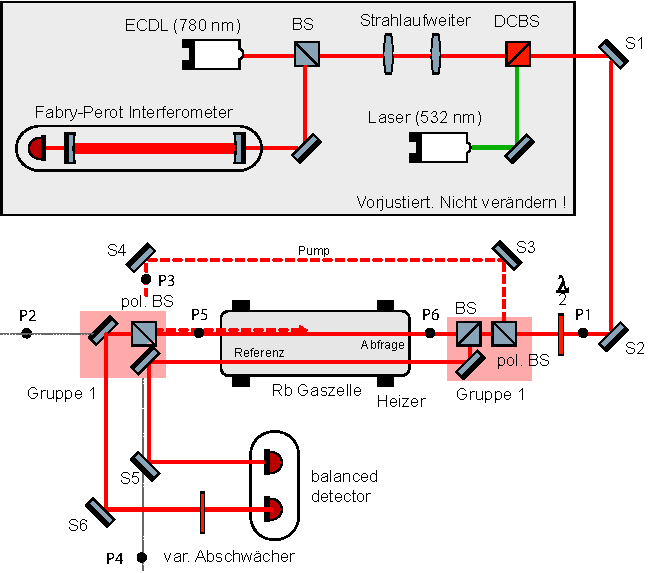
\includegraphics[width=\textwidth]{bilder/setup_rb.pdf}
   \caption{Versuchsaufbau. In den Baugruppen 1 und 2 sind die Elemente auf einer gemeinsamen Platte vorjustiert. Spiegel (S), Strahlteiler (BS), Farbteiler (DCBS), polarisierender Strahlteiler (pos. BS), Halbwellenplatte ($\lambda/2$) }
\end{figure}

Der Versuchsaufbau besteht aus einem vorjustierten Teil, der den Laser und das Fabry-Perot-Interferometer enthält. Dieser darf nicht verändert werden. Insbesondere die Überlagerung des grünen Justierlasers mit dem nahinfraroten Messlaser ist aufwendig. Das eigentliche Experiment bauen Sie ausgehend vom Spiegel S1 selbst auf. Dazu wird zunächst nur der grüne Justierlaser verwendet. Erst wenn alle Elemente damit justiert sind, schalten Sie den grünen Laser aus und den roten 780-nm-Laser ein. Vergessen Sie nicht, den grünen Laser während der eigentlichen Messung auszuschalten.

\paragraph{Anordnung} Es empfiehlt sich, die einzelnen Komponenten zunächst grob an der geplanten Position zu platzieren, um ein Gefühl für die Abstände zu bekommen. Um z.B. Leistungsmessungen durchführen zu können oder die Justierspitze platzieren zu können, ist es sinnvoll, die Optiken nicht zu dicht aneinander zu stellen. Merken Sie sich die Position und nehmen Sie dann alles wieder ab.

\paragraph{Strecke P1 -- P2} Die beiden Punkte P1 und P2 liegen auf einer Lochreihe und sind möglichst weit voneinander entfernt. Zuerst wird die Strecke P1 - P2 mit Hilfe der beiden Spiegel S1 und S2 wie oben beschrieben justiert. Der Strahlengang zwischen S1 und S2 ist unkritisch und muss nicht über die Justierspitze geführt werden. 

\paragraph{Wellenplatte und Baugruppe 1}  Stellen Sie die Wellenplatte und die Baugruppe 1 so in den Strahl P1--P2 ein, dass die Elemente nach Augenschein mittig und senkrecht getroffen werden.  Der abzweigende Pumpstrahl muss erst ab Punkt P3 wieder über einer Lochreihe laufen.

\paragraph{Strecke P3 -- P4} Justieren Sie den Pumpstrahl auf der Strecke P3--P4 mit den Spiegeln S3 und S4. Auf diese Weise kreuzen sich Pump- und Abfrage-Strahl senkrecht in einem Punkt.

\paragraph{Baugruppe 2, Punkte P5 und P6}  Stellen Sie  die Baugruppe 2 so auf, dass die reflektierende Innenfläche des Strahlteilers im Schnittpunkt der beiden Strahlen liegt und so der Punpstrahl möglichst genau entgegengesetzt zum  Abfragestrahl läuft. Blockieren Sie den durchlaufenen Abfrage- und Referenzstrahl nach der Baugruppe 1. Justieren Sie den Punkt P5 durch Verschieben der Baugruppen (ein Anschlag als Verschiebekante hilft hier!). Justieren Sie auf den Punkt P6 durch Verdrehen und Verkippen der Baugruppe 2. Iteriert Sie zwischen P5 und P6. Feinheiten lassen sich evtl. besser einstellen, wenn die Spiegel S3 und S4 verwendet werden. Dabei die Spiegel aber nur wenig verstellen, weil deren Position ja eigentlich schon gefunden ist.


\paragraph{Spiegel S5 und S6} Die Position dieser Spiegel ist unkritisch, solange sie sich nicht gegenseitig den Strahl blockieren. Lenken Sie die Strahlen wie gezeigt auf die  Detektorflächen.

\paragraph{Gaszelle} Stellen Sie die Rb Gaszelle so in den Strahlengang, dass Referenz- und Abfragestrahl ungestört transmittiert werden.


\paragraph*{Elektronik} Verbinden Sie den Detektor  mit der Datenerfassung (NI-USB 6002 AD-Interface) und den Heizer der Gaszelle mit seinem Netzteil. Schalten Sie den Heizer noch nicht ein.

\begin{margintable}
    \begin{tabular}{ll}
        Signal & Eingang \\
        Balanced Detector & AI 0 \\
        Monitor + & AI 1 \\
        50 Ohm Abschluss & AI 2 \\
        Monitor - & AI 3 \\
        Fabry-Perot-Diode & AI 4 \\
        Rückkanal Laser & AI 5
    \end{tabular}
    \caption{Belegung der Datenerfassung}
\end{margintable}

\paragraph*{Roter Laser} Jetzt sollte alles justiert sein. Schalten Sie den grünen Laser aus und  den roten Laser ein (zuerst den Controller oben links, dann links unten 'Laser on/off'). Stellen Sie mit Hilfe der Wellenplatte die Intensität in Pump- und Abfrage-Strahl so ein, dass beide im IR-Sichtgerät zu erkennen sind. Blockieren Sie den Pump-Strahl und stellen Sie an die Positionen P5 und P6 je eine Iris auf, die auf den Abfragestrahl zentriert ist. Benutzen Sie das Infrarotsichtgerät, um den roten Laserstrahl auf der Iris zu beobachten. Wenn die Iris justiert ist blockieren Sie  den Abfragestrahl und überprüfen, ob der Pumpstrahl von der anderen Seite jede Iris mittig trifft. Falls nicht, optimieren Sie die Iris an Stelle P5 mit Spiegel S3 und die an P6 mit Spiegel S4. Iterieren Sie über die beiden Spiegel bzw. Iris-Positionen. Um ein gutes Signal zu erhalten, muss diese Justage sehr genau erfolgen. Danach entfernen Sie die Iris wieder.


\begin{questions}
	\item 	 Wofür werden im Versuch zwei \emph{polarisierende} Strahlteilerwürfel benötigt? Wozu wird das $\lambda/ 2$-Plättchen gebraucht?
\end{questions}

\section{Programm zur Experimentsteuerung}


\begin{figure}
	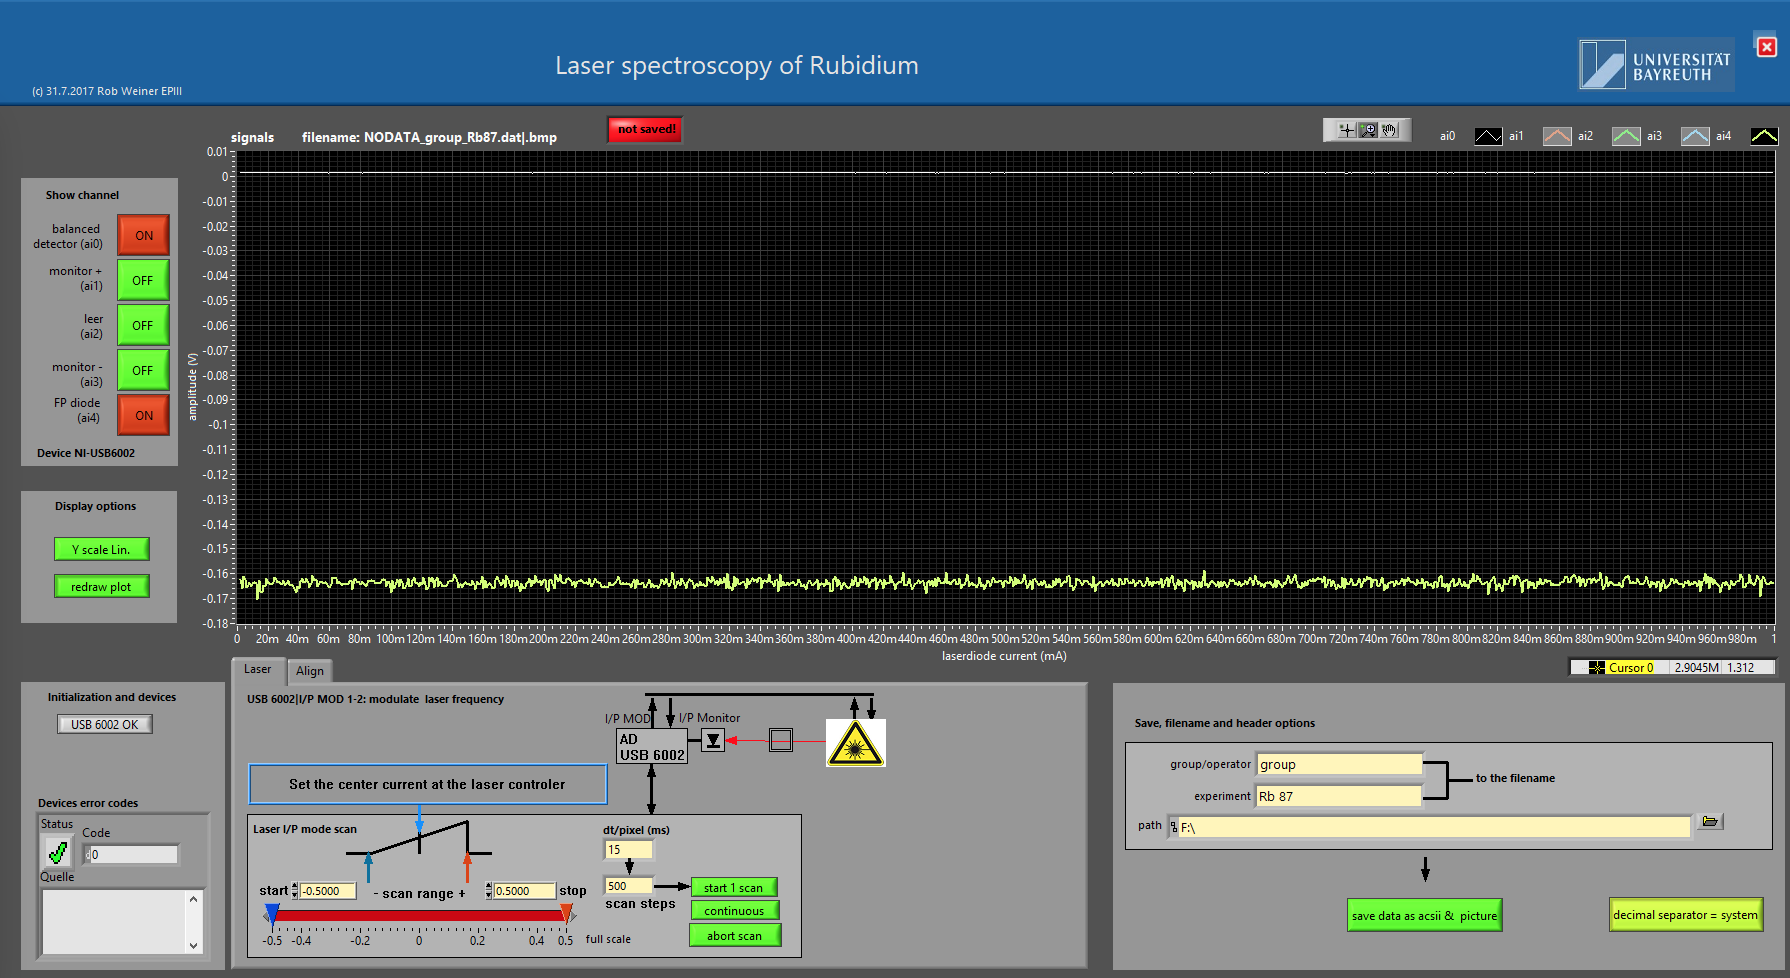
\includegraphics[width=\textwidth]{bilder/startansicht.png}
	\caption{Startansicht des Messprogramms.}
	\label{Startansicht Messprogramm}
\end{figure}


Starten Sie das Programm 'Rb Spektroskopie' auf dem Messrechner. Oben links können Sie die Signale der  Detektoren ein- und ausblenden. Aufgezeichnet und gespeichert wird immer alles. Unten links stellen Sie zwischen zwei Modi um: Messen und Justieren. Im Justier-Modus sehen Sie das Signal der eingeblendeten Detektoren als Funktion der Zeit durchlaufen. 
%XXX hier Nullen.XXX 
Im Modus 'Messen' wird der Laserwellenlänge variiert. Sie können die Anzahl der Datenpunkte ($< 20 \, 000$) und die Integrationszeit pro Datenpunkt ($> 15$ms) einstellen. Die aufgezeichneten Werte werden im großen Diagramm dargestellt und können mit dem Feld rechts unten gespeichert werden. Dabei sollten Sie sinnvolle Dateinamen vergeben. Die Daten werden als ASCII-Datensatz mit allen Kanälen sowie als Bildschirmfoto des angezeigten Graphen gespeichert.

Die Wellenlänge des Lasers wird, wie oben beschrieben, durch Verändern des Laserstroms variiert. Der Laser ist eigentlich dazu ausgelegt, seine Frequenz mit einer externen Elektronik auf eine der Rubidum-Linien zu stabilisieren. Daher verfügt er nur über einen schnellen, aber analogen Modulationseingang. Eine Spannung beeinflusst den am Controller eingestellten Strom. Der Zusammenhang Kontrollspannung--Strom ist dabei nicht völlig linear.

Im Messprogramm können Sie einen Verstellbereich des Stroms wählen, in Prozent eines Maximalbereichs, zentriert um die am Controller eingestellte Stromstärke. Dann wird eine passende Spannungsrampe abgefahren. Gleichzeitig wird der wirklich angelegte Strom über ein weiteres analoges Kontrollsignal des Laser ausgelesen. Das Signal dient zur Darstellung der horizontalen Strom-Achse.

Diese indirekte Arbeitsweise hat zwei Konsequenzen: Man kann das wirkliche abgefahrene Stromintervall nur ungenau einstellen. Es ist sinnvoll, sich langsam durch Variation des unteren und oberen Grenzwerts an die gewünschte Stellung heranzutasten. Weiterhin ist der zurückgelesene Stromwert rauschbehaftet, die Temperatur im Laser und damit seine Wellenlänge aber nicht. Sie sollten den angezeigten und gespeicherten Strom eines jeden Datenpunkts also nur zur Optimierung des Scanbereichs, jedoch nicht zur Bestimmung der Laserfrequenz benutzen.

Die Laserfrequenz ergibt sich aus dem Signal des Fabry-Perot-Interferometers. Sie können davon ausgehen, dass sich die Frequenz zwischen zwei Peaks des Interferometers monoton und linear verändert hat. Für die Berechnung ist lediglich die zeitliche Reihenfolge der Messwerte erforderlich, nicht jedoch der Stromwert selbst.


\section{Messungen}

\begin{marginfigure}[10mm]{\Huge \textbf{!}}\end{marginfigure}%
	Bringen Sie bitte einen USB-Stick zur Versuchsdurchführung mit, auf dem Sie Ihre Messdaten speichern und mitnehmen können.
Die Erfahrung zeigt, dass es einige Iterationen braucht, bis die beste Kombination der Parameter gefunden ist. Es ist daher sehr sinnvoll, die Daten bereits während des Versuchs zumindest soweit auszuwerten, dass Sie das Spektrum als Funktion der Frequenz darstellen können. So können Sie die gefundenen Linienpositionen mit den erwarteten vergleichen. 

% XXX braucht es Vorarbeiten, um peaks-Abweichungen zu bestimmen ?





\subsection{Doppler-verbreitertes Spektrum}

Stellen Sie mit Hilfe der Wellenplatte die Intensität des Abfragestrahls am Detektor so ein, dass der zugehörige Monitor-Ausgang ca. 1~Volt anzeigt. Der Pumpstrahl sollte nahezu die gesamte Leistung erhalten.

Für das Doppler-behaftete Spektrum reicht es auch, den Referenzstrahl zu betrachten. Lassen Sie sich Referenz-Leistung und Fabry-Perot-Diode anzeigen und scannen Sie die Laserfrequenz über den vollen Bereich. Sie müssen ein Strom-Intervall finden, in dem sich die vier Doppler-verbreiterten  Peaks des Hyperfeinspektrums im Absorptionssignal finden, und kein Modensprung dazwischen aufgetreten ist. Modensprünge erkennt man an unregelmäßigen Signalen im Fabry-Perot-Interferometer und leichten Sprüngen in der Ausgangsleistung, wie sie die Monitor-Ausgänge des Detektors abbilden. Suchen Sie zunächst nach dem 4-Peak-Spektrum, beseitigen Sie dann die Modensprünge durch Variation der Stromstärke und, nach Rücksprache mit dem Betreuer, der Peltier-Temperatur.

\subsection{Doppler-freies Spektrum}


Sorgen Sie  mit Hilfe eines variablen Abschwächers dafür, dass beide Dioden die gleiche Leistung sehen und so die Differenz Null wird. Das 'Nullen' des Balanced Detectors ist erforderlich, um eine optimale Unterdrückung des gemeinsamen Signals zu erreichen und das Differenzsignal untergrundfrei zu machen.

Nun sollten Sie ein Doppler-freies Spektrum im  Differenzsignal  finden. Optimieren Sie ggf. die Leistung im Pumpstrahl und auf den Photodioden. Optimieren Sie ggf. vorsichtig (!!) den Überlapp von Pump- und Abfragestrahl durch Spiegel S3 oder Verkippen von Baugruppe 2.

Achten Sie darauf, dass die einzelnen Monitor-Kanäle nicht sättigen, aber auch ausreichend Leistung vorhanden ist. Wählen Sie einen geeigneten Scanbereich, eine geeignete Integrationszeit und eine geeignete Pixelzahl.

Wenn alle Parameter richtig eingestellt sind, sollte die Abweichung zwischen der erwarteten und der beobachteten Linienposition nur wenige MHz betragen. Es kann jedoch sein, dass einige Linien nicht oder nur sehr schwach sichtbar sind. Dies ist bei der Zuordnung der Linien zu den Quantenzahlen zu berücksichtigen.

\subsection{Temperaturabhängigkeit}

Sie können die Temperatur der Rb-Gaszelle durch den Heizer variieren. Berücksichtigen Sie dabei, dass die Teilchenzahldichte exponentiell mit der Temperatur ansteigt (siehe Anhang). Die angezeigte Temperatur ist die des Heizelements, nicht notwendigerweise die des Gases. Auch ist Aufheizen einfacher und schneller als Abkühlen.



% show again from fromt	
\auftraege


Dokumentieren Sie Ihr Vorgehen und die ggf. von Ihnen zur Auswertung verwendenten (Python-)Skripte. Begründen Sie Ihre Entscheidungen. Diskutieren Sie die Ergebnisse, insbesondere wenn sie von Ihren Erwartungen abweichen.


	% Folgender Teil der Auswertung soll nur für eine Gaszellentemperatur durchgeführt werden, überlegen und begründen Sie, welche Gastemperatur Sie für die Auswertung benutzen.
	% \begin{enumerate}
	% 	\item Befreien Sie das Absorptionsspektrum von Trends und benennen Sie die Linien im Spektrum  mithilfe der jeweiligen Übergangsenergien.
		
	% 	\item Bestimmen Sie die Abstände der Energieniveaus des Absorptionsspektrums mithilfe des Fabry--Pérot--Interferometers--Signals als relativen Frequenzmaßstab. 
	% 	Stellen Sie diese mit entsprechender Frequenzachse graphisch dar.% vielleicht wären EV hier besser geeignet...
		
	% 	\item Berechnen Sie das tatsächliche Verhältnis der beiden Ru\-bi\-di\-um\-iso\-to\-pe in der Gaszelle. Schätzen Sie dazu die Gaußintegrale geeignet ab.
		
	% 	\item Stellen Sie das Doppler-freie Signal der vier Absorptionsdips einzeln dar und ordnen Sie die möglichen Energieübergänge zu. 
	% 	Fitten Sie für einen Absorptionsdip die Hyperfeindips mit Lorentzkurven. Was fällt Ihnen auf? 
	% 	Bestimmen Sie damit die Positionen und Abstände der einzelnen Dips. 
	% 	Vergleichen Sie diese anschließend mit den Literaturwerten der beigefügten Literatur.
	% 	(Gegebenfalls müssen Sie für diesen Aufgabenteil die Frequenzachse neu kalibrieren)
		
	% 	\item Bestimmen Sie die Hyperfeinstrukturkonstanten so weit wie möglich.
	
	% \end{enumerate}
	
	% Folgende Aufgabe sind für alle drei Gastemperaturen zu bearbeiten.
	
	% \begin{enumerate}
	% 	\item Berechnen Sie die verschiedenen Gastemperaturen und damit die Geschwindigkeiten des Gases mit Hilfe der gefitteten Gaußkurven des Absorptionsspektrums.
	% 	\item Vergleichen Sie Ihre Ergebnisse für die verschiedenen Gastemperaturen. 
	% \end{enumerate}
	

	% %---------------------

	% \section{Fragen zur Vorbereitung}
	
	% \begin{enumerate}
	% 	\item Warum sind die Kernspins der beiden Rubidiumisotope unterschiedlich? Welche Quantenzahlen existieren im Grundzustand und den ersten beiden angeregten Zuständen für die beiden Rubidiumisotope und welche F-Quantenzahlen resultieren daraus? 
		
	% 	\item Informieren Sie sich zu den Begriffen \glqq natürliche Linienbreite\grqq{}, \glqq Dop\-pler-Ver\-brei\-ter\-ung\grqq{}, \glqq homogene/inhomogene Verbreiterung\grqq{} und \glqq Sät\-ti\-gungs\-ver\-brei\-ter\-ung\grqq{}.
		
	% 	\item Was sind \glqq Cross-Over Resonanzen\grqq{} und wie entstehen diese?
		
	% 	\item Wofür werden im Versuch zwei Strahlteilerwürfel benötigt, die polarisierend sind? Wozu wird das $\lambda/ 2$-Plättchen und das Filterrad gebraucht?
		
	% 	\item Wie kann man aus den gewonnenen Daten die Hyperfeinstrukturkonstanten berechnen? Welche Hyperfeinübergänge sind im Spektrum zu erwarten?
	% \end{enumerate}
	



	%---------------------





%\end{document}	